\documentclass{article}
\usepackage[utf8]{inputenc}
\usepackage{url}
\usepackage[pdftex]{hyperref}
\usepackage{graphicx}

\begin{document}
\begin{titlepage}
   \begin{center}
        \vspace{3cm}

        \Huge{Cahier des besoins}

        \vspace{0.5cm}
        \LARGE{Analyse et représentation des sources Java}
            
        \vspace{3 cm}
    
        \vspace{1 cm}
        \Large{Encadrant}
        
        \vspace{0.25cm}
        \large{Thinhinane Yebda}
    
        \vspace{3 cm}
        \Large{Collaborateurs}
        
        \vspace{0.25cm}
        \large{Luigi Zaghet, Samuel Daugès, Paul Bourseau}
       
        \vspace{3 cm}
        \Large{Février 2022}
        
        \vspace{0.25 cm}
       

       \vfill
    \end{center}
\end{titlepage}

\tableofcontents

\section{Description du projet}
\subsection{Objet du projet}
Le projet qui nous a été confié consiste en un logiciel de refactoring et de re-engineering à partir de diagrammes de dépendances générés depuis le code.
\subsection{Définition des termes du projet}
Le Refactoring et le Reengineering est une activité d’ingénierie logicielle consistant à modifier le
code source d’une application de manière à améliorer sa qualité sans altérer son comportement vis-
à-vis des utilisateurs.\\
Le Reengineering est l’évaluation, l’analyse et l’altération d’une application existante dans le
but de le reconstituer sous une nouvelle forme, et la nouvelle implémentation de
l’application. Le processus englobe typiquement d’autres processus tels que le reverse
engineering, la redocumentation, le refactoring, et le post-engineering. Le but étant de
comprendre l’application existante (spécification, conception, implémentation) et de la
redévelopper sous une nouvelle forme. [1]\\
Le refactoring est le processus de restructuration et modification de l’application sans altérer
son comportement du code, mais en améliorant sa structure interne. [2]\\
Un diagramme de classe est un graphe destiné à illustrer les associations de dépendances entre classes d'objet. [4]\\
Dans la modélisation UML, une relation de dépendance est une relation dans laquelle une classe tire parti ou dépend d'une autre classe. [6]
\subsection{Présentation des collaborateurs}
Le projet sera réalisé par Samuel Daugès, Paul Bourseau et  Luigi Zaghet tout 3 étudiants en Master 1, semestre de Génie Logiciel et sous la supervision de Thinhinane Yebda ATER à l'université de Bordeaux.
\subsection{Prévisions des utilisateurs}
Les utilisateurs du logiciel seront des programmeurs java, que ce soit sur Linux, Windows ou Mac. Un portage sur Android ou IPhone ne sera pas nécessaire, rare sont les gens qui codent sur téléphone.
\section{Analyse de l'existant}
\subsection{Jdeps}
Jdeps est un analyseur de dépendances de classes java. Il permet d'afficher la liste des dépendances de classe dans un package ou une classe donné et dont le chemin est donné en paramètre. Il crée bel et bien un graphe de dépendance (possibilité de le sauvegarder dans un dossier au choix), mais il n'y a aucune option pour l'afficher (pas d'interface graphique, obligation de lire le fichier .dot dans un autre logiciel). De plus, il ne spécifie pas le type de dépendance. Enfin, jdeps ne traite que les fichiers compilés .class, et non les .java. Cela signifie qu'il est obligatoire de compiler avant de pouvoir l'utiliser, problème auquel nous pouvons remédier en analysant directement le code sources des fichiers .java [3]. Cependant, un gros avantage de jdeps est que cet outil vient directement avec l'installation de java, et qu'il s'utilise avec une simple commande dans le terminal.
\subsection{Poseidon for UML}
Poseidon for UML est un logiciel de modélisation pour l'Unified Modeling Language.
La version gratuite Community Edition gère les diagrammes UML, le re-engineering de code Java ainsi que la génération de code.[7] Le logiciel lit le code, le dessine en graphe UML puis permet de modifier le code. Poseidon supporte 9 diagrammes de la norme UML bien qu'il en existe 14 au total selon certaines sources.[8]

\section{Description des objectifs}
Analyse de sources de logiciels ou frameworks en Java
permettant l’extraction des graphes de dépendances entre
leurs composants (classes et paquetages).
Affichage de ces graphes de manière à apporter une aide à des
programmeurs qui voudraient agir sur ces programmes.
%(pour leur maintenance, extension, refactoring, etc.)

\section{Description des besoins}
\subsection{Liste de besoins fonctionnels}
    Les besoins principaux sont l'analyseur lexical permettant d'interpréter le code, ainsi que la création du graphe de dépendances. Les deux devront travailler ensemble afin de réaliser la conversion du code source en diagramme UML par exemple.\\
    Il est possible d'obtenir le graphe des dépendances à partir de l'analyse du code source (code java), ou du bytecode [3]. Il faudrait donc créer un analyseur grammatical capable de lire les noms de classe, ainsi que le code source java dans l'idéal. L'idée principale serait que notre programme puisse prendre en entrée un fichier java non compilé, et reconnaisse les différentes instanciations et implémentations de classe afin de déterminer correctement les dépendances sans avoir à compiler. Pour cela, il faut être capable d'identifier les différents mots clés, tels que "extends", "implements", ou les noms de classes, qui auront été déterminés en listant les noms des fichiers java dans le package. Le fait de pouvoir créer ce graphe de dépendances avant la compilation permettrait de repérer des erreurs de façon prématurée. %(par exemple, une classe A qui a comme attribut une instance de la classe B, et une classe B qui a comme attribut une instance de la classe A).
    Une fois le code traduit par l'analyseur grammatical, il faut l'afficher sous forme de graphes UML en affichant les 14 types de diagrammes UML.[8]
\subsection{Liste de besoins non fonctionnels}
    -Contraintes / difficultés : complexité en temps de la conversion en graphe, "lisibilité" du code source.\\
    -Risques éventuels : mauvaise compréhension du code par l'analyseur, qui peut créer et conserver des erreurs dans la nouvelle version du code.\\
    -Outils de repérages des designs patterns et possibilités d'ajout de ces derniers quand du code leur ressemble.\\
    -Tester la fonctionnalité en reprenant le graphe issu du programme,  le convertissant en code java, puis en comparant les deux codes.\\
    -Interface simple et facile à prendre en main pour l'utilisateur.\\
    -Possibilité de modifications du code à partir du diagramme de dépendance.\\
    
    
\section{Organisation du Projet}
\subsection{Lecture du code par l'analyseur}
La première étape sera de créer un analyseur lexical qui prends seulement les informations qui lui sont utiles afin de créer un diagramme UML par la suite (voir 5.3), soit les variables, leurs noms et leurs types ainsi que les fonctions, leurs noms, leurs types et leurs paramètres et le type de ces derniers. Pour cela quatres classes seront créé:\\
-la classe \emph{Variable} qui a comme variable un String qui sera le nom, ainsi qu'un autre String qui correspondra à son type.\\
-la classe \emph{Function} qui contient son nom en format String, son type sous le même format ainsi qu'une liste de \emph{Variable} correspondant à ses paramètres.\\
-la classe \emph{Class} qui contient une liste de \emph{Variable} et une liste de \emph{Function}.\\
-la classe \emph{Classes} qui correspond à un liste de \emph{Class} afin de toutes les garder dans une seule variable.\\
\subsection{Préparation de la mise en diagramme UML}
Une fois toutes les classes enregistrés indépendamment les unes des autres, il faut maintenant repérer les dépendances entre les classes, les types de diagrammes et éventuellement des designs patterns. Pour se faire une nouvelle classe sera créer, \emph{Dependencies} qui définie les dépendances d'une classe et dont une liste serait présente dans la classe \emph{Class}. La classe \emph{Dependencies} contiendra une variable \emph{Class} et son type définit par un énum sachant qu'il existe seulement 4 types d'injection de dépendances (constructeur, interface, mutateur et champs[10]).
On remarque que le code actuel ressemble au code utilisé pour l'affichage de graphes avec les \emph{Class} qui sont les sommets et leur dépendances qui sont leurs voisins.
\subsection{Affichage du Diagramme UML}
La classe \emph{Application} qui possèdera une variable \emph{Classes}, sera composée de deux méthodes permettant la création et l'affichage du diagramme UML.\\
La première méthode consistera à lire la liste des classes soit la partie 5.1 ainsi que les dépendances et les liens entre elles soit la partie 5.2. %puis de les écrire en langage "PlantUML" dans un nouveau fichier en format ".puml".[11]\\
%La seconde méthode consistera simplement à afficher les fichier nouvellement créer.
Il faut ensuite afficher le diagramme UML qui peut s'apparenter à un graphe, la bibliothèque qui sera utilisés est JGraphX qui permet de dessiner des graphes en 2D.[12] Le programme commencera par initialiser un String puis parcourir la liste des classes, récupérera son nom, l'ajoutera au String, même chose pour les variables et les fonctions en prenant également leur attribut, le String final constituera le nom du graphes pour un sommet. Une fois ceci fait pour toutes les classes, le programme parcours une nouvelle fois la liste des ces dernières afin de récupérer leurs dépendances et d'ajouter des arrêtes entre les sommets nommer d'après de le type d'injection de dépendances. Quand tout cela est fait, le graphe final est affiché et le programmeur peut voir son programme sous forme de diagramme UML.

\subsection{Récapitulatif et rôles}
Le diagramme UML du logiciel a été donné en guise de récapitulatif.\\
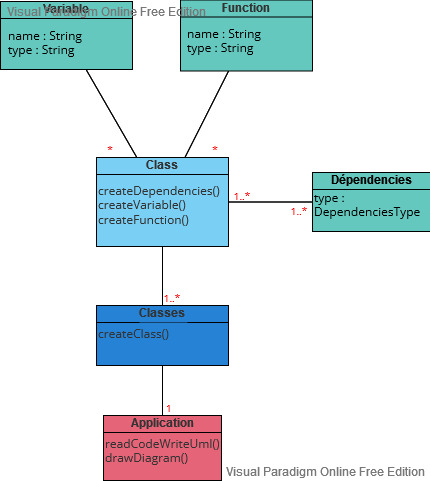
\includegraphics[width=12cm]{PdpUml.jpg}\\
L'organisation du projet a été réparti en 3 sous-parties:\\ -la première partie, lecture du code par l'analyseur constitue le début de la fonction \emph{readCodeWriteUml()} soit la partie \emph{readCode()} ainsi que les classes \emph{Classes}, \emph{Class}, \emph{Variable}, \emph{Function}, \emph{Dependencies}. La création de ces classes peut être réparti afin d'équilibrer la charge de travail. Sinon l'écriture du code de cette partie sera Samuel Daugès.\\
-la deuxième partie, préparation de la mise en Diagramme UML constitue la suite de la fonction WriteUML(), cette partie sera écrite par Luigi Zaghet.\\
-la troisième et dernière partie consitue la fonction drawDiagram() de la classe \emph{Application}, cette partie sera écrite par Paul Bourseau.\\
\begin{thebibliography}{9}
\bibitem{def refactoring} "Qu'est-ce que le refactoring ?" \href{https://www.ionos.fr/digitalguide/sites-internet/developpement-web/quest-ce-que-le-refactoring/}{ionos.fr}, Digital Guide IONOS, 29 Sept 2020, consulté le 31 Janv 2022.

\bibitem{def reengineering} "Réingénierie : définition dans le glossaire logistique"
\href{https://www.faq-logistique.com/Definition-Reingenierie.htm}{faq-logistique.com}, FAQ Logistique, consulté le 31 Janv 2022.

\bibitem{article graphe dépendance}
Dietrich, J., Yakovlev, V., McCartin, C., Jenson, G., Duchrow, M. (2008, September). Cluster analysis of Java dependency graphs. In Proceedings of the 4th ACM symposium on Software visualization (pp. 91-94).

\bibitem{def diagramme de dépendance}"Fiche du terme : Diagramme de dépendance"
\href{http://www.thesaurus.gouv.qc.ca/tag/terme.do?id=MDL420}{thesaurus.gouv.qc.ca}, Gouvernement du Québec, consulté le 31 Janv 2022.

\bibitem{exemple de ce qu'on veut faire} "Java reverse engineering - Eclipse" \href{https://wiki.eclipse.org/Java_reverse_engineering}{eclipse.org}, Eclipse Foundation, consulté le 31 Janv 2022.

\bibitem{définition dépendances}Relation de dépendances - Documentation IBM \href{https://www.ibm.com/docs/fr/rsm/7.5.0?topic=diagrams-dependency-relationships}{www.ibm.com}, consulté le 06 Fevr 2022.

\bibitem{Poseidon for UML}Présentation de Gentleware Poseidon CE 2.x.
\href{https://wpetrus.developpez.com/uml/poseidon/}{wpetrus.developpez.com}, consulté le 06 Fevr 2022.

\bibitem{14 diagrammes UML à utiliser}UML Diagrams Types
\href{https://creately.com/blog/diagrams/uml-diagram-types-examples/}{creately.com}, consulté le 06 Fevr 2022.

\bibitem{Cours sur l'analyse lexicale}Forax R, Constant M, Chilowicz M, "Analyse lexicale, Analyse syntaxique" cours de l'Université Marne La Vallée, consulté le 07 Fevr 2022.

\bibitem{Les types d'injection de dépendances}Introduction à l'injection de dépendance en Java
\href{https://zestedesavoir.com/tutoriels/309/introduction-a-linjection-de-dependances-en-java/}{zestedesavoir.com}, consulté le 07 Fevr 2022.

\bibitem{Création d'un diagramme UML}Présentation de l'extension PlantUML
\href{https://plantuml.com/fr/class-diagram}{plantuml.com}, consulté le 07 Fevr 2022.

\bibitem{JGraph pour l'affichage des graphes}JGraphx: Les bases
\href{https://pbriand.developpez.com/tutoriels/java/JGraphX/les-bases/#L2}{pbriand.developpez.com}, consulté le 08/02/2022.

\end{thebibliography}

\end{document}